% id: 44-13
% book: 100발100중 3-2 중간 · 01 3-2 중간(삼각비·삼각비의 활용·원과 직선·원주각·부록)
% section: 실전문제 1회 서술형 문제
% figure: crop:fig-44-13.png
% answer: $39\mkern3mu \mathrm{m}$
% answer_source: 답지(빠른정답)
% variant_level: 0 (원본 전사)
% 이 파일은 build.mjs 가 items.json 에서 만든다. 고칠 때는 items.json 을 고친다.
\smash{\raisebox{1.5mm}{\dmkichul{100발100중 3-2 중간 44쪽 13번 · 출제유력}}}
\noindent\begin{minipage}[t]{0.58\linewidth}\vspace{0pt}\raggedright 그림과 같이 민수의 눈높이는 $1.8\mkern3mu \mathrm{m}$이고, 기둥의 꼭대기인 $\pt{C}$지점을 올려다본 각의 크기는 $43^\circ$이다. 두 지점~$\pt{A}$와 $\pt{B}$ 사이의 거리가 $40\mkern3mu \mathrm{m}$일 때, 기둥의 높이를 구하고, 그 과정을 서술하시오. (단, $\tan 43^\circ=0.93$으로 계산한다.) \mbox{[5점]}\end{minipage}\hfill\begin{minipage}[t]{0.4\linewidth}\vspace{0pt}\centering 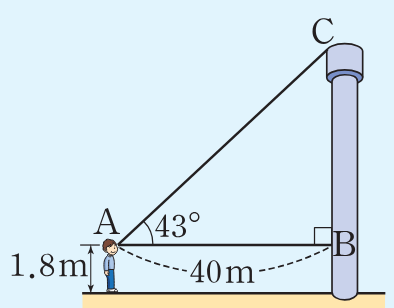
\includegraphics[width=94.4pt]{figures/fig-44-13.png}\end{minipage}\par
